% CalendarBot -- Deliverable 3 (one vertical page). Editorial layout; same navy/teal/gold palette as Deliverables 1 and 2.
% Compile with pdfLaTeX (MiKTeX: inter + plex packages); check that it stays on one page.
% Every number comes from numeros.tex, generated by hacer_numeros.py from the Colab results.
\documentclass[10pt,a4paper]{article}
\usepackage[a4paper,left=0.42in,right=0.42in,top=0.3in,bottom=0.4in,footskip=0.2in]{geometry}
\usepackage[T1]{fontenc}
\usepackage[utf8]{inputenc}
\usepackage[sfdefault,semibold,scale=0.92]{inter}
\usepackage[scale=0.86]{plex-mono}
\usepackage{amssymb}
\usepackage{graphicx}
\usepackage[table]{xcolor}
\usepackage{booktabs}
\usepackage{array}
\usepackage{tabularx}
\usepackage{microtype}
\usepackage{tikz}
\usetikzlibrary{positioning,arrows.meta,calc,fit,backgrounds}
\usepackage[skins]{tcolorbox}
\usepackage{enumitem}
\usepackage{fancyhdr}
\usepackage{hyperref}

% ---------- palette (same as Deliverables 1 and 2) ----------
\definecolor{navy}{HTML}{173B57}
\definecolor{teal}{HTML}{087E8B}
\definecolor{pale}{HTML}{F3F8F9}
\definecolor{gold}{HTML}{C9A227}
\definecolor{bad}{HTML}{B5473A}
\definecolor{ink}{HTML}{22313F}
\definecolor{mute}{HTML}{6B7A86}
\definecolor{line}{HTML}{D5DEE3}
% one colour per failure family: it threads sections 01, 04 and the heat map
\colorlet{fdur}{gold}
\colorlet{fdate}{teal}
\colorlet{fpart}{bad}

\newcommand{\videourl}{https://youtu.be/VIDEO_ID}   % open video link
\newcommand{\repourl}{https://github.com/maty20arriagada/SML-GEN-AI-for-Calendar-services}
\newcommand{\f}[1]{\texttt{#1}}
\newcommand{\lbl}[1]{{\bfseries\tiny\color{teal}\MakeUppercase{#1}}\par\vspace{1pt}}
\newcommand{\dotc}[1]{{\color{#1}\raisebox{0.15ex}{\scalebox{0.9}{$\bullet$}}}}
\newcommand{\tagf}[2]{\tcbox[on line, colback=#1!9, colframe=#1!9, arc=0.8mm, boxsep=0pt, left=2pt, right=2pt, top=0.6pt, bottom=0.6pt, boxrule=0pt, fontupper=\tiny\color{#1!70!black}]{\dotc{#1}\,#2}}
\newcommand{\Fdur}{\tagf{fdur}{reminder read as duration}}
\newcommand{\Fdate}{\tagf{fdate}{dates, hours, time zones}}
\newcommand{\Fpart}{\tagf{fpart}{participants invented}}
\newcommand{\stopm}{\leavevmode{\color{bad}\rule[0.05ex]{0.55em}{0.55em}}}
% heat-map cell: share correct of set B class, white -> teal
% \mk{...} flags the cell a sentence of the text points at (gold)
\newif\ifheatmark
\newcommand{\heatcell}[2]{\edef\heatP{\the\numexpr(#1*100)/#2\relax}%
  \edef\heatC{\noexpand\cellcolor{teal!\the\numexpr(#1*82)/#2+4\relax!white}}%
  \ifheatmark\def\heatC{\cellcolor{gold}}\fi\heatC
  \makebox[0.52cm]{\ifheatmark\color{navy}\bfseries\else\ifnum\heatP>55 \color{white}\bfseries\else\color{ink}\fi\fi #1/#2}}
\newcommand{\mk}[1]{\heatmarktrue#1\heatmarkfalse}

\newcommand{\setres}[3]{\expandafter\def\csname R#1#2\endcsname{#3}}
\newcommand{\R}[2]{\csname R#1#2\endcsname}
\setres{E0}{A}{1 (1\%)}
\setres{E0}{B}{4 (10\%)}
\setres{E0}{C}{0 (0\%)}
\setres{E0}{T}{5 (3\%)}
\setres{E1}{A}{82 (88\%)}
\setres{E1}{B}{20 (49\%)}
\setres{E1}{C}{17 (65\%)}
\setres{E1}{T}{119 (74\%)}
\setres{E4}{A}{88 (95\%)}
\setres{E4}{B}{38 (93\%)}
\setres{E4}{C}{21 (81\%)}
\setres{E4}{T}{147 (92\%)}
\setres{E4T1}{A}{68 (73\%)}
\setres{E4T1}{B}{32 (78\%)}
\setres{E4T1}{C}{20 (77\%)}
\setres{E4T1}{T}{120 (75\%)}
\setres{E4T2}{A}{88 (95\%)}
\setres{E4T2}{B}{38 (93\%)}
\setres{E4T2}{C}{21 (81\%)}
\setres{E4T2}{T}{147 (92\%)}
\setres{E4T3}{A}{88 (95\%)}
\setres{E4T3}{B}{38 (93\%)}
\setres{E4T3}{C}{21 (81\%)}
\setres{E4T3}{T}{147 (92\%)}
\setres{E4T4}{A}{86 (92\%)}
\setres{E4T4}{B}{34 (83\%)}
\setres{E4T4}{C}{19 (73\%)}
\setres{E4T4}{T}{139 (87\%)}
\setres{E4T5}{A}{88 (95\%)}
\setres{E4T5}{B}{38 (93\%)}
\setres{E4T5}{C}{21 (81\%)}
\setres{E4T5}{T}{147 (92\%)}
\newcommand{\setpct}[3]{\expandafter\def\csname P#1#2\endcsname{#3}}\newcommand{\PCT}[2]{\csname P#1#2\endcsname}
\setpct{E0}{A}{1}
\setpct{E0}{B}{10}
\setpct{E0}{C}{0}
\setpct{E0}{T}{3}
\setpct{E1}{A}{88}
\setpct{E1}{B}{49}
\setpct{E1}{C}{65}
\setpct{E1}{T}{74}
\setpct{E4}{A}{95}
\setpct{E4}{B}{93}
\setpct{E4}{C}{81}
\setpct{E4}{T}{92}
\setpct{E4T1}{A}{73}
\setpct{E4T1}{B}{78}
\setpct{E4T1}{C}{77}
\setpct{E4T1}{T}{75}
\setpct{E4T2}{A}{95}
\setpct{E4T2}{B}{93}
\setpct{E4T2}{C}{81}
\setpct{E4T2}{T}{92}
\setpct{E4T3}{A}{95}
\setpct{E4T3}{B}{93}
\setpct{E4T3}{C}{81}
\setpct{E4T3}{T}{92}
\setpct{E4T4}{A}{92}
\setpct{E4T4}{B}{83}
\setpct{E4T4}{C}{73}
\setpct{E4T4}{T}{87}
\setpct{E4T5}{A}{95}
\setpct{E4T5}{B}{93}
\setpct{E4T5}{C}{81}
\setpct{E4T5}{T}{92}
\newcommand{\setcls}[4]{\expandafter\def\csname CLS#1#2\endcsname{\heatcell{#3}{#4}}}\newcommand{\cls}[2]{\csname CLS#1#2\endcsname}
\setcls{E0}{duracion_vs_recordatorio}{0}{7}
\setcls{E0}{weekday_numero}{0}{4}
\setcls{E0}{fecha_invalida}{4}{4}
\setcls{E0}{ingles_relativo}{0}{5}
\setcls{E0}{rol_compuesto}{0}{5}
\setcls{E0}{complemento_titulo}{0}{6}
\setcls{E0}{ampm}{0}{5}
\setcls{E0}{control}{0}{5}
\setcls{E1}{duracion_vs_recordatorio}{7}{7}
\setcls{E1}{weekday_numero}{0}{4}
\setcls{E1}{fecha_invalida}{1}{4}
\setcls{E1}{ingles_relativo}{0}{5}
\setcls{E1}{rol_compuesto}{3}{5}
\setcls{E1}{complemento_titulo}{2}{6}
\setcls{E1}{ampm}{2}{5}
\setcls{E1}{control}{5}{5}
\setcls{E4}{duracion_vs_recordatorio}{7}{7}
\setcls{E4}{weekday_numero}{4}{4}
\setcls{E4}{fecha_invalida}{4}{4}
\setcls{E4}{ingles_relativo}{4}{5}
\setcls{E4}{rol_compuesto}{3}{5}
\setcls{E4}{complemento_titulo}{6}{6}
\setcls{E4}{ampm}{5}{5}
\setcls{E4}{control}{5}{5}
\setcls{E4T1}{duracion_vs_recordatorio}{6}{7}
\setcls{E4T1}{weekday_numero}{2}{4}
\setcls{E4T1}{fecha_invalida}{4}{4}
\setcls{E4T1}{ingles_relativo}{4}{5}
\setcls{E4T1}{rol_compuesto}{2}{5}
\setcls{E4T1}{complemento_titulo}{6}{6}
\setcls{E4T1}{ampm}{4}{5}
\setcls{E4T1}{control}{4}{5}
\setcls{E4T2}{duracion_vs_recordatorio}{7}{7}
\setcls{E4T2}{weekday_numero}{4}{4}
\setcls{E4T2}{fecha_invalida}{4}{4}
\setcls{E4T2}{ingles_relativo}{4}{5}
\setcls{E4T2}{rol_compuesto}{3}{5}
\setcls{E4T2}{complemento_titulo}{6}{6}
\setcls{E4T2}{ampm}{5}{5}
\setcls{E4T2}{control}{5}{5}
\setcls{E4T3}{duracion_vs_recordatorio}{7}{7}
\setcls{E4T3}{weekday_numero}{4}{4}
\setcls{E4T3}{fecha_invalida}{4}{4}
\setcls{E4T3}{ingles_relativo}{4}{5}
\setcls{E4T3}{rol_compuesto}{3}{5}
\setcls{E4T3}{complemento_titulo}{6}{6}
\setcls{E4T3}{ampm}{5}{5}
\setcls{E4T3}{control}{5}{5}
\setcls{E4T4}{duracion_vs_recordatorio}{7}{7}
\setcls{E4T4}{weekday_numero}{4}{4}
\setcls{E4T4}{fecha_invalida}{4}{4}
\setcls{E4T4}{ingles_relativo}{4}{5}
\setcls{E4T4}{rol_compuesto}{3}{5}
\setcls{E4T4}{complemento_titulo}{2}{6}
\setcls{E4T4}{ampm}{5}{5}
\setcls{E4T4}{control}{5}{5}
\setcls{E4T5}{duracion_vs_recordatorio}{7}{7}
\setcls{E4T5}{weekday_numero}{4}{4}
\setcls{E4T5}{fecha_invalida}{4}{4}
\setcls{E4T5}{ingles_relativo}{4}{5}
\setcls{E4T5}{rol_compuesto}{3}{5}
\setcls{E4T5}{complemento_titulo}{6}{6}
\setcls{E4T5}{ampm}{5}{5}
\setcls{E4T5}{control}{5}{5}
\newcommand{\setdelta}[3]{\expandafter\def\csname D#1#2\endcsname{#3}}
\newcommand{\dlt}[2]{\csname D#1#2\endcsname}
\setdelta{E0}{A}{$-$87}
\setdelta{E0}{B}{$-$34}
\setdelta{E0}{C}{$-$21}
\setdelta{E0}{T}{$-$142}
\expandafter\def\csname BLE0\endcsname{4.26cm}
\setdelta{E1}{A}{$-$6}
\setdelta{E1}{B}{$-$18}
\setdelta{E1}{C}{$-$4}
\setdelta{E1}{T}{$-$28}
\expandafter\def\csname BLE1\endcsname{0.84cm}
\setdelta{E4}{A}{0}
\setdelta{E4}{B}{0}
\setdelta{E4}{C}{0}
\setdelta{E4}{T}{0}
\expandafter\def\csname BLE4\endcsname{0.00cm}
\setdelta{E4T1}{A}{$-$20}
\setdelta{E4T1}{B}{$-$6}
\setdelta{E4T1}{C}{$-$1}
\setdelta{E4T1}{T}{$-$27}
\expandafter\def\csname BLE4T1\endcsname{0.81cm}
\setdelta{E4T2}{A}{0}
\setdelta{E4T2}{B}{0}
\setdelta{E4T2}{C}{0}
\setdelta{E4T2}{T}{0}
\expandafter\def\csname BLE4T2\endcsname{0.00cm}
\setdelta{E4T3}{A}{0}
\setdelta{E4T3}{B}{0}
\setdelta{E4T3}{C}{0}
\setdelta{E4T3}{T}{0}
\expandafter\def\csname BLE4T3\endcsname{0.00cm}
\setdelta{E4T4}{A}{$-$2}
\setdelta{E4T4}{B}{$-$4}
\setdelta{E4T4}{C}{$-$2}
\setdelta{E4T4}{T}{$-$8}
\expandafter\def\csname BLE4T4\endcsname{0.24cm}
\setdelta{E4T5}{A}{0}
\setdelta{E4T5}{B}{0}
\setdelta{E4T5}{C}{0}
\setdelta{E4T5}{T}{0}
\expandafter\def\csname BLE4T5\endcsname{0.00cm}
\newcommand{\dlen}[1]{\csname BL#1\endcsname}
\newcommand{\nA}{93}\newcommand{\nB}{41}\newcommand{\nC}{26}\newcommand{\nT}{160}
\newcommand{\pValT}{$p<0.001$}\newcommand{\fixT}{31}\newcommand{\brokT}{3}
\newcommand{\pValC}{$p=0.219$}\newcommand{\fixC}{5}\newcommand{\brokC}{1}
\newcommand{\setchg}[2]{\expandafter\def\csname CHG#1\endcsname{#2}}\newcommand{\chg}[1]{\csname CHG#1\endcsname}
\setchg{E4T1}{37}
\setchg{E4T2}{0}
\setchg{E4T3}{0}
\setchg{E4T4}{8}
\setchg{E4T5}{0}
\newcommand{\fallbackrate}{0\%}\newcommand{\loopsrate}{4\%}
\newcommand{\triagerej}{0}\newcommand{\corrN}{55}\newcommand{\corrRej}{45}
\newcommand{\vramA}{8.74}\newcommand{\vramE}{8.12}\newcommand{\vramD}{0.62}
\newcommand{\failinput}{\f{"Dinner with Tom at 7 pm New York time on October 9"} {\color{mute}(set C, id 20)}}
\newcommand{\failwhy}{The phrase carried every value; three gaps lined up. \f{extraer\_zona\_horaria} knows only Madrid and Argentina and \emph{silently} returns the Santiago default instead of \f{null}. A3 trusted the tool over the phrase and spent its steps re-asking it, so the date tool was never called. A4 saw the wrong zone but chose \f{corregir} on a field outside its bounded fixes instead of returning the work to A3: no invented value got in, but the loop that would have caught it was not taken.}



\hypersetup{colorlinks=true,urlcolor=teal,linkcolor=teal,pdftitle={CalendarBot: from a pipeline to four agents}}
\setlength{\parskip}{0.1em}
\setlength{\parindent}{0pt}
\emergencystretch=2em
\setlength{\tabcolsep}{3pt}
\renewcommand{\arraystretch}{1.0}
\setlist{nosep,leftmargin=0.9em,itemsep=1pt,topsep=1pt,label={\color{teal}\tiny$\blacktriangleright$}}
\color{ink}

% ---------- section heading: big gold number, navy title, hairline, rubric criterion on the right ----------
\newcommand{\sect}[3]{\par\vspace{3.5pt}\noindent
  \begin{tikzpicture}[baseline=(n.base)]
    \node[anchor=base west, inner sep=0pt, font=\fontsize{15}{15}\selectfont\bfseries, text=gold] (n) at (0,0) {#1};
    \node[anchor=base west, inner sep=0pt, font=\small\bfseries, text=navy] (t) at ([xshift=5pt]n.base east) {#2};
    \node[anchor=base east, inner sep=0pt, font=\tiny, text=mute] (r) at (\linewidth,0) {\MakeUppercase{rubric $\cdot$ #3}};
    \draw[line, line width=0.5pt] ([xshift=6pt, yshift=2.2pt]t.base east) -- ([xshift=-6pt, yshift=2.2pt]r.base west);
  \end{tikzpicture}\par\vspace{2.5pt}}

\pagestyle{fancy}
\fancyhf{}
\renewcommand{\headrulewidth}{0pt}
\fancyfoot[C]{\parbox{\textwidth}{\centering
  {\color{gold}\rule{\textwidth}{0.4pt}}\par\vspace{1pt}
  {\tiny\color{mute}GAI 580694 \;$\cdot$\; Universidad de Concepci\'on \;$\cdot$\; Deliverable 3 \;$\cdot$\; Due: October 31, 2026, 23:59}}}

\begin{document}
\scriptsize

% ================= HEADER =================
\noindent
\begin{tikzpicture}
\fill[navy, rounded corners=1.6mm] (0,0) rectangle (\textwidth, 1.45cm);
\fill[gold] (0,0) rectangle (\textwidth, 0.05cm);
\node[anchor=north west, text=white, align=left, inner sep=0pt] at (0.38cm, 1.24cm) {
  {\fontsize{16.5}{17}\selectfont\bfseries CalendarBot: from a pipeline to four agents}\\[3pt]
  {\tiny\color{white!75!navy} Generative Artificial Intelligence (580694) \,$\cdot$\, Universidad de Concepci\'on \,$\cdot$\, Spring 2026}\\[1pt]
  {\tiny Mat\'ias Arriagada \,$\cdot$\, Cristian C\'ardenas \,$\cdot$\, Pablo Silva \,$\cdot$\, Daniela Vidal}};
\node[anchor=east, fill=white, rounded corners=1.2mm, inner sep=2.5pt] at (\textwidth-0.3cm, 0.75cm)
  {
\includegraphics[height=0.62cm]{marcaderecha.png}};
\end{tikzpicture}

\vspace{3pt}\noindent{\tiny
{\bfseries\color{teal}REPO}\; \href{\repourl}{github.com/maty20arriagada/SML-GEN-AI-for-Calendar-services}\hfill
{\bfseries\color{teal}PROMPTS}\; one versioned file per agent in \f{deliverable3/prompts/}\hfill
{\bfseries\color{teal}TRACES}\; every input, \f{resultados/traces/}\hfill
{\bfseries\color{gold!85!black}VIDEO}\; \href{\videourl}{open link (3 min)}}

% ================= KPI STRIP =================
\vspace{4pt}\noindent
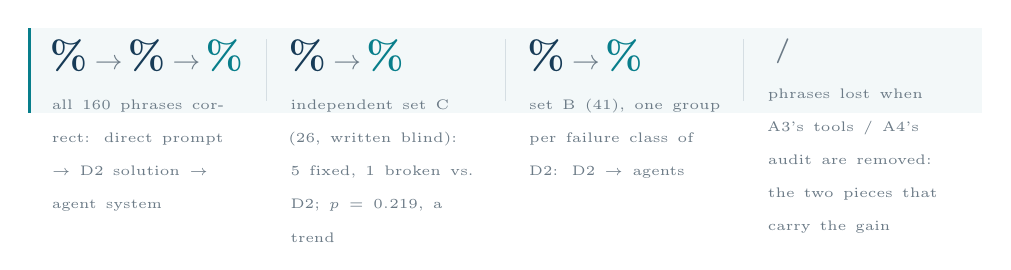
\begin{tikzpicture}
\fill[pale] (0,0) rectangle (\textwidth, 1.08cm);
\fill[teal] (0,0) rectangle (1.2pt, 1.08cm);
\foreach \i in {1,2,3} \draw[line] ({\i*\textwidth/4}, 0.15cm) -- ({\i*\textwidth/4}, 0.93cm);
\newcommand{\kpi}[3]{\node[anchor=north west, align=left, inner sep=0pt, text width=\textwidth/4-0.6cm] at ({#1*\textwidth/4+0.3cm}, 0.94cm)
  {{\fontsize{15.5}{16}\selectfont\bfseries\color{navy}#2}\\[2.5pt]{\tiny\color{mute}#3}};}
\kpi{0}{\PCT{E0}{T}\%{\color{mute}\,\normalsize$\to$\,}\PCT{E1}{T}\%{\color{mute}\,\normalsize$\to$\,}{\color{teal}\PCT{E4}{T}\%}}{all \nT\ phrases correct: direct prompt $\to$ D2 solution $\to$ agent system}
\kpi{1}{\PCT{E1}{C}\%{\color{mute}\,\normalsize$\to$\,}{\color{teal}\PCT{E4}{C}\%}}{independent set C (\nC, written blind): \fixC\ fixed, \brokC\ broken vs.\ D2; \pValC, a trend}
\kpi{2}{\PCT{E1}{B}\%{\color{mute}\,\normalsize$\to$\,}{\color{teal}\PCT{E4}{B}\%}}{set B (\nB), one group per failure class of D2: D2 $\to$ agents}
\kpi{3}{{\color{bad}\dlt{E4T1}{T}}{\color{mute}\,\small /\,}{\color{bad}\dlt{E4T4}{T}}}{phrases lost when A3's tools / A4's audit are removed: the two pieces that carry the gain}
\end{tikzpicture}

% ================= 01 CONTINUITY =================
\sect{01}{The task, the failure and the criterion we kept}{continuity with D1--D2}
\begin{minipage}[t]{0.315\linewidth}\lbl{Same task, same criterion}
A Spanish/English chat phrase becomes a 9-field calendar event. \emph{Correct} = every scored field matches the ground truth (\f{evaluar.py}, 8 fields; \f{recurrence} not scored), \f{null}/\f{[]} when absent, nothing invented; relative dates from 2026-09-01. Unchanged since D1.
\end{minipage}\hfill{\color{line}\vrule width 0.4pt}\hfill
\begin{minipage}[t]{0.315\linewidth}\lbl{The failure D2 left open}
D2 (Qwen3-4B + LoRA + date resolver) reached \PCT{E1}{A}\% on its own benchmark but still broke on three families:\\[1.5pt]
\Fdur\ ``avísame 15 min antes''\\[1pt]
\Fdate\ ``31/09'', ``viernes 18'', ``7 pm'', ``horario de Madrid''\\[1pt]
\Fpart\ ``ensayo de la \underline{banda}'' $\to$ \f{["banda"]}
\end{minipage}\hfill{\color{line}\vrule width 0.4pt}\hfill
\begin{minipage}[t]{0.315\linewidth}\lbl{Declared deviations}
Four agents on the \emph{same} open model (Qwen3-4B-Instruct + LoRA \f{checkpoint-300}, merged). \nT\ phrases instead of \nA: \textbf{A} (\nA, the D2 benchmark, where errors were diagnosed: optimistic), \textbf{B} (\nB, validation by failure class built after the error analysis, not independent), \textbf{C} (\nC, written blind).
\end{minipage}

% ================= 02 GRAPH =================
\sect{02}{Four agents, one model: who decides what happens next}{agent graph}
\centering
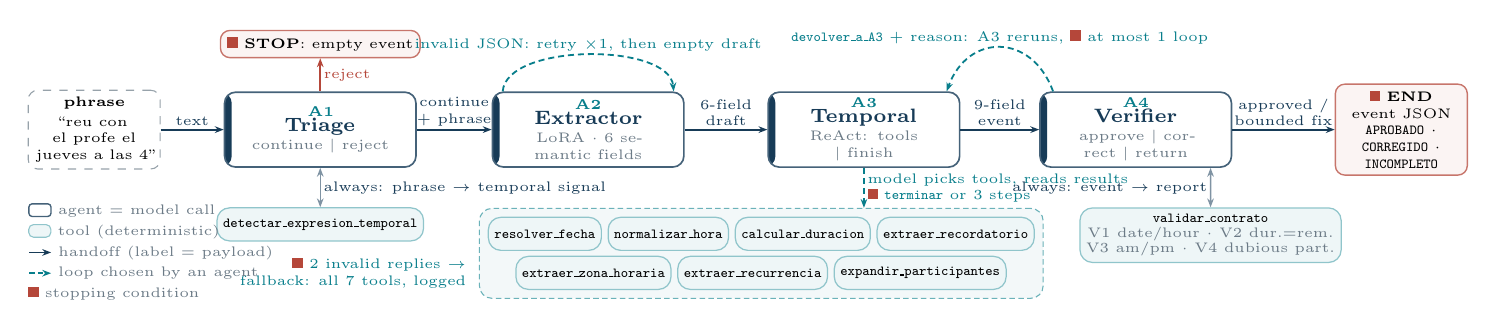
\begin{tikzpicture}[
  font=\tiny, >={Stealth[length=3.2pt]}, node distance=0.95cm,
  ag/.style={draw=navy!80, rounded corners=1.4mm, fill=white, align=center, minimum height=0.95cm, text width=2.15cm, inner ysep=2.2pt, inner xsep=4pt, line width=0.6pt,
    path picture={\fill[navy] (path picture bounding box.north west) rectangle ([xshift=2.6pt]path picture bounding box.south west);}},
  tl/.style={draw=teal!45, rounded corners=1.6mm, fill=teal!7, align=center, minimum height=0.42cm, inner sep=2.2pt, line width=0.45pt, font=\ttfamily\tiny},
  io/.style={draw=mute!70, dashed, rounded corners=1.2mm, fill=white, align=center, inner sep=2.5pt},
  stp/.style={draw=bad!75, rounded corners=1.2mm, fill=bad!6, align=center, inner sep=2.5pt, line width=0.5pt},
  ar/.style={->, draw=navy, line width=0.65pt},
  fx/.style={<->, draw=navy!55, line width=0.5pt},
  lp/.style={->, draw=teal, line width=0.65pt, dash pattern=on 2.2pt off 1.4pt},
  lab/.style={font=\tiny, inner sep=1pt, text=navy}]
\newcommand{\agn}[3]{{\color{teal}\bfseries #1}\\[-0.5pt]{\scriptsize\bfseries\color{navy}#2}\\[0.5pt]{\color{mute}#3}}
\node[io, text width=1.5cm] (in) {\bfseries phrase\\[1pt]\mdseries``reu con el profe el jueves a las 4''};
\node[ag, right=0.8cm of in] (a1) {\agn{A1}{Triage}{continue $\mid$ reject}};
\node[ag, right=of a1] (a2) {\agn{A2}{Extractor}{LoRA $\cdot$ 6 semantic fields}};
\node[ag, right=1.05cm of a2] (a3) {\agn{A3}{Temporal}{ReAct: tools $\mid$ finish}};
\node[ag, right=1.0cm of a3] (a4) {\agn{A4}{Verifier}{approve $\mid$ correct $\mid$ return}};
\node[stp, right=1.3cm of a4, text width=1.5cm] (out) {\stopm\ \textbf{END}\\event JSON\\{\ttfamily APROBADO $\cdot$ CORREGIDO $\cdot$ INCOMPLETO}};
\draw[ar] (in) -- node[lab, above] {text} (a1);
\draw[ar] (a1) -- node[lab, above, align=center] {continue\\+ phrase} (a2);
\draw[ar] (a2) -- node[lab, above, align=center] {6-field\\draft} (a3);
\draw[ar] (a3) -- node[lab, above, align=center] {9-field\\event} (a4);
\draw[ar] (a4) -- node[lab, above, align=center] {approved /\\bounded fix} (out);
\node[stp, above=0.42cm of a1] (rej) {\stopm\ \textbf{STOP}: empty event};
\draw[ar, draw=bad] (a1) -- node[lab, right, text=bad] {reject} (rej);
\draw[lp] ([xshift=4pt]a2.north west) .. controls +(0.05,0.62) and +(-0.05,0.62) .. node[lab, above, text=teal] {invalid JSON: retry $\times$1, then empty draft} ([xshift=-4pt]a2.north east);
\draw[lp] ([xshift=5pt]a4.north west) to[out=110,in=70,looseness=1.5] node[lab, above, text=teal] {\f{devolver\_a\_A3} + reason: A3 reruns, \stopm\ at most 1 loop} ([xshift=-5pt]a3.north east);
% tools: one node each
\node[tl, below=0.5cm of a1] (t0) {detectar\_expresion\_temporal};
\node[tl, below=0.5cm of a4, xshift=0.95cm] (t4) {validar\_contrato\\[-0.5pt]\rmfamily\color{mute}V1 date/hour $\cdot$ V2 dur.=rem.\\[-0.5pt]\rmfamily\color{mute}V3 am/pm $\cdot$ V4 dubious part.};
\node[tl, below=0.62cm of a2, xshift=-0.55cm] (r1) {resolver\_fecha};
\node[tl, right=0.07cm of r1] (r2) {normalizar\_hora};
\node[tl, right=0.07cm of r2] (r3) {calcular\_duracion};
\node[tl, right=0.07cm of r3] (r4) {extraer\_recordatorio};
\node[tl, below=0.06cm of r1.south west, anchor=north west, xshift=0.35cm] (r5) {extraer\_zona\_horaria};
\node[tl, right=0.07cm of r5] (r6) {extraer\_recurrencia};
\node[tl, right=0.07cm of r6] (r7) {expandir\_participantes};
\begin{scope}[on background layer]
\node[draw=teal!60, dash pattern=on 2pt off 1.2pt, rounded corners=1.6mm, fill=pale, inner sep=3pt, fit=(r1)(r4)(r5)(r7)] (t3) {};
\end{scope}
\draw[fx] (a1) -- node[lab, right] {always: phrase $\to$ temporal signal} (t0);
\draw[<->, lp] (a3.south) -- node[lab, right, text=teal, align=left] {model picks tools, reads results\\\stopm\ \f{terminar} or 3 steps} (a3.south |- t3.north);
\node[lab, text=teal, anchor=east, align=right] at ($(t3.west |- r5)+(-0.12,0)$) {\stopm\ 2 invalid replies $\to$\\fallback: all 7 tools, logged};
\draw[fx] ($(a4.south)+(0.95,0)$) -- node[lab, left] {always: event $\to$ report} ($(t4.north)$);
% legend
\node[anchor=north west, inner sep=0pt, align=left, text=mute] at ($(in.south west)+(0,-0.42)$) {
  \tikz[baseline=-0.6ex]\draw[navy!80, fill=white, line width=0.5pt, rounded corners=0.4mm] (0,-0.07) rectangle (0.28,0.09); agent = model call\\[1.5pt]
  \tikz[baseline=-0.6ex]\draw[teal!45, fill=teal!7, rounded corners=0.6mm] (0,-0.07) rectangle (0.28,0.09); tool (deterministic)\\[1.5pt]
  \tikz[baseline=-0.6ex]\draw[navy, ->, line width=0.6pt] (0,0) -- (0.28,0); handoff (label = payload)\\[1.5pt]
  \tikz[baseline=-0.6ex]\draw[teal, ->, line width=0.6pt, dash pattern=on 2pt off 1.2pt] (0,0) -- (0.28,0); loop chosen by an agent\\[1.5pt]
  \stopm\ stopping condition};
\end{tikzpicture}\par
\raggedright

% ================= 03 AGENT DESIGN =================
\sect{03}{Why four roles: the work is split by the kind of error, not by the code}{agent design}
{\renewcommand{\arraystretch}{1.12}\setlength{\tabcolsep}{4.5pt}
\begin{tabularx}{\linewidth}{@{}>{\bfseries\color{navy}}l >{\raggedright\arraybackslash}X >{\raggedright\arraybackslash}p{5.9cm} >{\raggedright\arraybackslash}p{3.75cm}@{}}
\arrayrulecolor{navy}\toprule\arrayrulecolor{line}
 & \textbf{Role the task needs, and why no other agent covers it} & \textbf{Receives $\to$ returns \;{\color{mute}$\cdot$ prompt file}} & \textbf{Stops / hands off}\\
\midrule
A1 & \emph{Is this an event at all?} The only agent that can end a run, so an unusable reply means continue. & phrase + temporal signal $\to$ \f{\{accion, razon, idioma\}} \;{\color{mute}\f{a1\_triage\_v2.txt}} & \stopm\ reject: empty event; else $\to$ A2\\
A2 & \emph{Semantic fields}: what the D2 LoRA already does well. It sees no dates, so its habits cannot corrupt them. & phrase $\to$ 6-field JSON \;{\color{mute}\f{a2\_extractor\_v1.txt}} & valid $\to$ A3; invalid: retry once\\
A3 & \emph{Time reasoning.} Tools resolve dates and pm hours where a 4B model slips; only the model knows which ones a phrase needs. & phrase, A2 draft, ref.\ date, A4 objection $\to$ \f{\{pensamiento, accion, tools\}} per step \;{\color{mute}\f{a3\_agente\_v1.txt}} & \stopm\ \f{terminar}, 3 steps or 2 invalid replies $\to$ A4\\
A4 & \emph{Independent audit.} A model misses its own errors; a second reading against phrase and contract catches them. Only A4 can send work back. & phrase, event, \f{validar\_contrato} report $\to$ \f{\{razonamiento, accion, correcciones\}} \;{\color{mute}\f{a4\_agente\_v1.txt}} & approve / correct $\to$ END; return $\to$ A3, \stopm\ once\\
\arrayrulecolor{navy}\bottomrule
\end{tabularx}}

% ================= 04 TECHNIQUES =================
\sect{04}{What each technique buys: removed one at a time, traced to the failure it targets}{prompting techniques}
\begin{minipage}[t]{0.605\linewidth}\vspace{0pt}
{\renewcommand{\arraystretch}{1.12}
\newcommand{\eff}[1]{\leavevmode{\color{bad}\rule[-0.4pt]{\dlen{#1}}{4.2pt}}\,\textbf{\dlt{#1}{T}}\,{\color{mute}(C\,\dlt{#1}{C})}}
\begin{tabularx}{\linewidth}{@{}l >{\raggedright\arraybackslash}X r@{}}
\arrayrulecolor{navy}\toprule\arrayrulecolor{line}
\textbf{Technique} {\color{mute}$\cdot$ agent} & \textbf{Failure it targets} & \textbf{Effect of removing it: all {\color{mute}(C)}}\\
\midrule
\textbf{T1} tool use, model picks tools {\color{mute}$\cdot$ A3} & \Fdate & \eff{E4T1}\\
\textbf{T2} contrastive few-shot {\color{mute}$\cdot$ A4} & \Fpart & \eff{E4T2}\\
\textbf{T3} rubric + step-by-step {\color{mute}$\cdot$ A4} & \Fpart\ \Fdur & \eff{E4T3}\\
\textbf{T4} verifier + return loop {\color{mute}$\cdot$ A4} & \Fpart\ A3's blind spots & \eff{E4T4}\\
\textbf{T5} triage gate {\color{mute}$\cdot$ A1} & non-events, malformed input & \eff{E4T5}\\
\arrayrulecolor{navy}\bottomrule
\end{tabularx}}\par\vspace{3pt}
\textbf{Reading.} Two techniques carry the gain. Without \textbf{T1}, \chg{E4T1} outputs change and the date classes slip (weekday + number 4/4 $\to$ 2/4). Without \textbf{T4}, title complement falls from 6/6 to 2/6: the verifier is what keeps ``ensayo de la banda'' from inventing a participant. \textbf{T2, T3, T5 measure zero}, and the traces say why: A1 never rejected (no phrase is a non-event) and \corrRej\ of A4's \corrN\ corrections hit a field it may not fix, so A4's wording rarely reaches the output. Loop A4$\to$A3 in \loopsrate\ of runs; A3 fallback \fallbackrate.
\end{minipage}\hfill
\begin{minipage}[t]{0.37\linewidth}\vspace{0pt}
{\bfseries\tiny\color{teal}SET B, CORRECT PER FAILURE CLASS}\par\vspace{2pt}
{\tiny\setlength{\tabcolsep}{2.2pt}\renewcommand{\arraystretch}{1.42}
\newcommand{\hrow}[2]{#1 & \cls{E0}{#2} & \cls{E1}{#2} & \cls{E4}{#2} & \cls{E4T1}{#2} & \cls{E4T4}{#2}\\}
\newcommand{\hrowT}[2]{#1 & \cls{E0}{#2} & \cls{E1}{#2} & \cls{E4}{#2} & \mk{\cls{E4T1}{#2}} & \cls{E4T4}{#2}\\}
\newcommand{\hrowF}[2]{#1 & \cls{E0}{#2} & \cls{E1}{#2} & \cls{E4}{#2} & \cls{E4T1}{#2} & \mk{\cls{E4T4}{#2}}\\}
\begin{tabular}{@{}l *{5}{c}@{}}
 & \textbf{E0} & \textbf{E1} & \textbf{E4} & \textbf{$-$T1} & \textbf{$-$T4}\\[1pt]
\hrow{\dotc{fdur}\,reminder read as duration}{duracion_vs_recordatorio}
\hrowT{\dotc{fdate}\,weekday + day number}{weekday_numero}
\hrow{\dotc{fdate}\,impossible date (31/09)}{fecha_invalida}
\hrow{\dotc{fdate}\,English relative date}{ingles_relativo}
\hrow{\dotc{fdate}\,am/pm hour}{ampm}
\hrowF{\dotc{fpart}\,title complement}{complemento_titulo}
\hrow{\dotc{fpart}\,compound role}{rol_compuesto}
\hrow{\dotc{mute}\,control (no trap)}{control}
\end{tabular}}\par\vspace{2pt}
{\tiny\color{mute}E0 direct prompt, E1 D2 solution, E4 agents, $-$T$k$ ablations; {\color{gold!80!black}\bfseries gold} = the drops named in the reading. B was built after the error analysis: it shows \emph{where} each piece acts, not how well the system generalises.}
\end{minipage}

% ================= 05 EVIDENCE =================
\sect{05}{Evidence: same \nT\ inputs, same criterion (all scored fields correct) for every arm}{evidence of improvement}
\begin{minipage}[t]{0.555\linewidth}\vspace{0pt}
{\renewcommand{\arraystretch}{1.05}
\begin{tabular}{@{}l r r r >{\columncolor{gold!14}}r r r@{}}
\arrayrulecolor{navy}\toprule\arrayrulecolor{line}
\textbf{Arm} & \textbf{A} & \textbf{B} & \textbf{C} & \textbf{All} & \textbf{$\Delta$C} & \textbf{$\Delta$All}\\
{\color{mute}$\Delta$ = vs.\ E4} & {\color{mute}n=\nA} & {\color{mute}n=\nB} & {\color{mute}n=\nC} & {\color{mute}n=\nT} & & \\
\midrule
E0 \; direct prompt, base model & \R{E0}{A} & \R{E0}{B} & \R{E0}{C} & \R{E0}{T} & \dlt{E0}{C} & \dlt{E0}{T}\\
E1 \; D2 solution & \R{E1}{A} & \R{E1}{B} & \R{E1}{C} & \R{E1}{T} & \dlt{E1}{C} & \dlt{E1}{T}\\
\rowcolor{teal!9} \textbf{\color{navy}E4 \; full agent system} & \textbf{\R{E4}{A}} & \textbf{\R{E4}{B}} & \textbf{\R{E4}{C}} & \textbf{\R{E4}{T}} & ref. & ref.\\
E4 $-$ T1 tools (A3) & \R{E4T1}{A} & \R{E4T1}{B} & \R{E4T1}{C} & \R{E4T1}{T} & \dlt{E4T1}{C} & \dlt{E4T1}{T}\\
E4 $-$ T2 few-shot (A4) & \R{E4T2}{A} & \R{E4T2}{B} & \R{E4T2}{C} & \R{E4T2}{T} & \dlt{E4T2}{C} & \dlt{E4T2}{T}\\
E4 $-$ T3 rubric/CoT (A4) & \R{E4T3}{A} & \R{E4T3}{B} & \R{E4T3}{C} & \R{E4T3}{T} & \dlt{E4T3}{C} & \dlt{E4T3}{T}\\
E4 $-$ T4 verifier + loop & \R{E4T4}{A} & \R{E4T4}{B} & \R{E4T4}{C} & \R{E4T4}{T} & \dlt{E4T4}{C} & \dlt{E4T4}{T}\\
E4 $-$ T5 triage (A1) & \R{E4T5}{A} & \R{E4T5}{B} & \R{E4T5}{C} & \R{E4T5}{T} & \dlt{E4T5}{C} & \dlt{E4T5}{T}\\
\arrayrulecolor{navy}\bottomrule
\end{tabular}}
\end{minipage}\hfill
\begin{minipage}[t]{0.425\linewidth}\vspace{0pt}
\begin{tikzpicture}[x=0.0335cm, y=0.36cm, font=\tiny]
\foreach \v in {0,25,50,75,100} {\draw[line, line width=0.3pt] (\v,0.45) -- (\v,-3.5); \node[text=mute, anchor=north] at (\v,-3.5) {\v\%};}
\newcommand{\drow}[3]{%
  \node[anchor=east, text=navy, align=right] at (-3,#2) {\bfseries #3};
  \draw[line width=1.6pt, teal!25] (\PCT{E1}{#1},#2) -- (\PCT{E4}{#1},#2);
  \fill[mute!55] (\PCT{E0}{#1},#2) circle (2.1pt);
  \fill[gold] (\PCT{E1}{#1},#2) circle (2.3pt);
  \fill[navy] (\PCT{E4}{#1},#2) circle (2.5pt);
  \node[anchor=west, text=navy, font=\tiny\bfseries] at (\PCT{E4}{#1}+2.5,#2) {\PCT{E4}{#1}};}
\drow{A}{0}{A, diagnosed}
\drow{B}{-1}{B, by class}
\drow{C}{-2}{C, blind}
\drow{T}{-3}{All \nT}
\node[anchor=south west, align=left, text=mute] at (-3,0.55) {\tikz\fill[mute!55] circle (2pt); E0 direct \quad \tikz\fill[gold] circle (2pt); E1 D2 \quad \tikz\fill[navy] circle (2pt); E4 agents};
\end{tikzpicture}\par\vspace{1pt}
\textbf{Paired test vs.\ D2 (exact McNemar).} Independent set C: E4 fixes \fixC\ phrases E1 failed and breaks \brokC, \pValC: \emph{a trend, not proof} with n\,=\,\nC. All \nT: \fixT\ fixed, \brokT\ broken, \pValT; A is optimistic and B is not independent, so C is the number we stand behind.
\end{minipage}\par\vspace{3pt}
{\bfseries\tiny\color{teal}HARDWARE (MEASURED)}\;\; {\tiny Colab free $\cdot$ Tesla T4 15.6 GB $\cdot$ fp16 \;{\color{line}|}\; Qwen3-4B-Instruct + LoRA (merged) for every agent \;{\color{line}|}\; peak VRAM \vramA\ GB agents vs.\ \vramE\ GB direct prompt (+\vramD\ GB)}\par\vspace{1pt}
{\bfseries\tiny\color{bad}LIMITS}\;\; {\tiny A1/A2 outputs are cached and shared by all arms, so ablations differ only downstream \;{\color{line}|}\; only C is blind \;{\color{line}|}\; n is small, one checkpoint \;{\color{line}|}\; A1 untested on real non-events}

% ================= 06 FAILURE =================
\sect{06}{Where it still breaks: a real failure, read from its trace}{failure case}
\begin{minipage}[t]{0.5\linewidth}\vspace{0pt}
\begin{tcolorbox}[enhanced, colback=pale, colframe=pale, boxrule=0pt, arc=1.2mm, left=4pt, right=4pt, top=3pt, bottom=3pt,
  borderline west={1.2pt}{0pt}{bad}]
{\tiny\renewcommand{\arraystretch}{1.08}\setlength{\tabcolsep}{2.5pt}
\newcommand{\who}[1]{{\bfseries\color{navy}#1}}
\begin{tabularx}{\linewidth}{@{}l >{\raggedright\arraybackslash}X@{}}
\who{in} & \failinput\\
\who{A1} & \f{detectar\_expresion\_temporal} $\to$ \f{fecha 2026-10-09} {\color{teal}\checkmark}; \f{continuar}\\
\who{A2$\to$A3} & \f{\{titulo: Dinner, hora: 19:00, participantes: [Tom]\}} {\color{teal}\checkmark}\\
\who{A3 step 1} & \f{normalizar\_hora} $\to$ \f{19:00}; \f{extraer\_zona\_horaria} $\to$ {\color{bad}\f{America/Santiago}}\\
\who{A3 steps 2--3} & \f{extraer\_zona\_horaria} again, same answer; \stopm\ step cap. {\color{bad}\f{resolver\_fecha} never called}\\
\who{A4} & \f{validar\_contrato} $\to$ \f{[]}; ``timezone must be New York'' $\to$ \f{corregir}: {\color{bad}rejected}\\
\who{out} & \leavevmode{\color{bad}\bfseries INCOMPLETO}: \f{fecha=null}, \f{zona\_horaria=America/Santiago} (6/8 fields)\\
\end{tabularx}}
\end{tcolorbox}
\end{minipage}\hfill
\begin{minipage}[t]{0.475\linewidth}\vspace{0pt}
\lbl{Why it fails}
\failwhy\ {\color{mute}Trace: \f{traces/falla/}; video inputs: \f{traces/video/}.}
\end{minipage}

\end{document}
